% LaTeX source for ``การเรียนรู้ของเครื่องสำหรับเคมีควอนตัม (Machine Learning for Quantum Chemistry)''
% Copyright (c) 2022 รังสิมันต์ เกษแก้ว (Rangsiman Ketkaew).

% License: Creative Commons Attribution-NonCommercial-NoDerivatives 4.0 International (CC BY-NC-ND 4.0)
% https://creativecommons.org/licenses/by-nc-nd/4.0/

\chapter{การทำนายคุณสมบัติของโมเลกุล}
\label{ch:predict_molprop}

\begin{figure}[htbp]
    \centering
    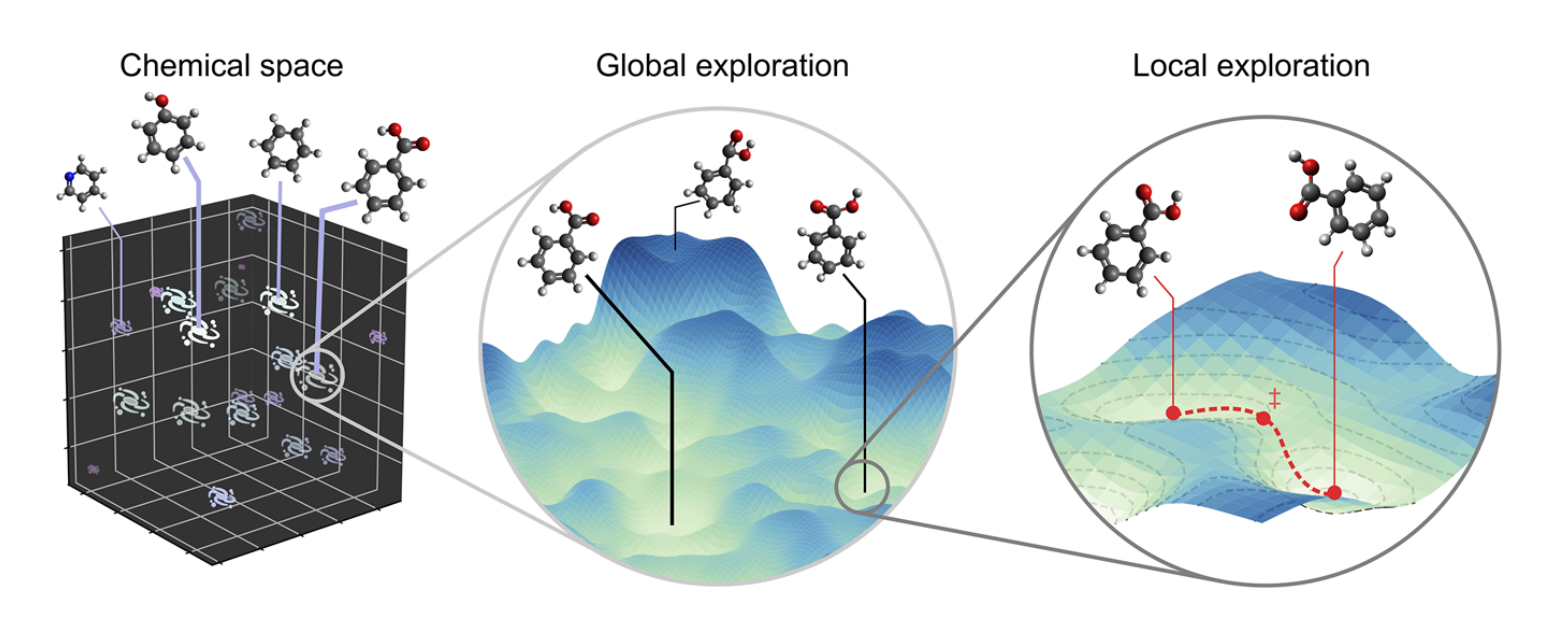
\includegraphics[width=\linewidth]{fig/ml_pred_chem.png}
    \caption{การสำรวจคุณสมบัติเชิงโมเลกุลในปริภูมิเชิงเคมีแบบ Local และ Global 
    (เครดิตภาพ: \textit{J. Chem. Phys.} 2021, 154, 230903 \autocite{westermayr2021b})}
    \label{fig:ml_pred_chem}
\end{figure}

ในบทนี้เราจะมาศึกษาการทำนายสมบัติของโมเลกุลด้วย ML ซึ่งถือได้ว่าเป็นหัวใจสำคัญของส่วนที่สองของหนังสือเล่มนี้เลยก็ว่าได้ โดยผู้อ่านจะได้%
เรียนรู้และทำความเข้าใจลำดับขั้นตอนในการใช้โมเดล ML ในการทำนายคุณสมบัติเชิงอิเล็กทรอนิกส์ทางควอนตัมต่าง ๆ ที่ได้ศึกษาไปแล้วในบทที่ 
\ref{ch:el_prop} ซึ่งเป้าหมายหลักของการทำวิจัยในสาขานี้ก็คือการศึกษาและพัฒนา Representation และโมเดล ML ที่สามารถทำนาย%
คุณสมบัติเชิงควอนตัมของโมเลกุลที่ต้องการได้อย่างแม่นยำและเทียบเคียงได้กับผลจากการคำนวณด้วยวิธีเคมีควอนตัมแบบมาตรฐาน เช่น วิธี DFT 
และวิธีเชิงฟังก์ชันคลื่น\autocite{ceriotti2018} นอกจากนี้ผู้อ่านจะได้ศึกษาตัวอย่างโค้ดที่สามารถนำไปใช้งานในการทำนายได้จริงซึ่งผู้เขียน%
เชื่อว่าการศึกษาทฤษฎีควบคู่ไปพร้อมกับการเขียนโปรแกรมนั้นจะช่วยทำให้เข้าใจทฤษฎีได้อย่างถูกต้องและรวดเร็วเพราะการเขียนโปรแกรมช่วยให้เรา%
คิดอย่างเป็นระบบและเข้าใจสิ่งที่ศึกษาอย่างเป็นขั้นเป็นตอน
\idxboth{การทำนายคุณสมบัติของโมเลกุล}{Molecular Property Prediction}

%--------------------------
\section{แนวทางการปฏิบัติ}
\label{sec:pred_best_prac}
%--------------------------

แนวทางปฏิบัติ (Best Practice) หรือลำดับขั้นตอนสำหรับการนำ ML มาประยุกต์กับเคมีควอนตัมสามารถแบ่งออกเป็น 6 ขั้นตอนง่าย ๆ ได้ดังนี้
\idxen{Best Practice}

\begin{enumerate}
    \item วิเคราะห์ชุดข้อมูลดิบและทำความสะอาดข้อมูล (Data Analysis และ Data Cleaning)
    
    \item เลือก Representation/Descriptor ที่จะนำมาคำนวณ Feature 
    
    \item เลือกอัลกอริทึม ML ที่เหมาะสมกับโจทย์ของเรา 
    
    \item ฝึกสอนโมเดลและทำนายคำตอบ
    
    \item ศึกษาผลกระทบจากการเปลี่ยน Hyperparameter และทำ Validation
    
    \item ประเมินประสิทธิภาพของโมเดลและวิเคราะห์ผลการทำนาย
\end{enumerate}

ขั้นตอนแรกของการนำ ML มาประยุกต์กับเคมีควอนตัมก็คือการเตรียมข้อมูลดิบ (Raw Data) นั่นก็คือข้อมูลทางเคมีเบื้องต้นของโมเลกุลที่เรามี 
โดยส่วนใหญ่แล้วนักเคมีเชิงคำนวณมักจะเริ่มต้นด้วยการเตรียม Cartesian Coordinates ของชุดโมเลกุลที่ต้องการศึกษา เช่น โมเลกุลอินทรีย์
สารประกอบโลหะ ฯลฯ เมื่อเรามีชุดข้อมูลแล้วสิ่งที่เราควรทำต่อไปก็คือการวิเคราะห์ข้อมูลแบบเชิงลึก (Exploratory Data Analysis หรือ EDA) 
ซึ่งในขั้นตอนนี้เราควรจะต้องทำความสะอาดข้อมูลดิบด้วย เช่น การนำค่าผิดปกติออกไป การแปลงพารามิเตอร์บางค่าให้อยู่ในรูปแบบที่เหมาะสม 
โดยเราสามารถใช้เทคนิค Unsupervised ML เช่น Elliptic Envelope, Isolation Forest, และ Local Outlier Factor (LOF)
ในการตรวจหาค่าผิดปกติได้
\idxen{Best Practice!Data Analysis}
\idxen{Best Practice!Data Cleaning}

ลำดับถัดมาคือเราจะต้องเลือก Representation หรือ Descriptor ที่เราต้องการนำมาคำนวณมาคุณสมบัติต่าง ๆ ของโมเลกุล 
ซึ่งเรามักจะได้มาจากการคำนวณด้วยวิธีแบบดั้งเดิม โดยการคำนวณ Representation นั้นก็จะมีให้เลือกมากมาย ขึ้นอยู่กับความสอดคล้องของอินพุต 
(Feature ที่เราคำนวณ) กับเอาต์พุตที่เราต้องการจะทำนาย ซึ่งขั้นตอนนี้จะเป็นการสร้าง Feature Vector สำหรับการฝึกโมเดล ML นั่นเอง 
เมื่อเราได้ชุดข้อมูลที่มี Input Feature แล้ว อาจจะมีขั้นตอนที่เพิ่มเข้ามาเพื่อช่วยให้เราเข้าใจชุดข้อมูลได้มากขึ้น เช่น เราอาจจะใช้วิธีทางสถิติเข้า%
มาช่วยคำนวณค่าทางสถิติของชุดข้อมูลก่อนนำไปฝึกสอนโมเดล เช่น ค่าเฉลี่ย (Mean), ค่าเบี่ยงเบน (Deviation), การแจกแจงความถี่, 
(Frequency), ความแปรปรวน (Variance), และสหสัมพันธ์ของเพียร์สัน (Pearson Correlation) ซึ่งค่าทางสถิติเหล่านี้จะช่วยให้เข้าใจการ%
กระจายตัวในชุดข้อมูลรวมไปถึงความสำคัญ (Importance) ของ Feature แต่ละตัวในชุดข้อมูล ซึ่งนำไปสู่การตัดสินใจและวิเคราะห์ว่า Feature 
ตัวไหนที่น่าจะมีผลต่อประสิทธิภาพของโมเดลเรามากที่สุด 

เมื่อเราได้ชุดข้อมูลที่มีความเหมาะสมแล้ว ขั้นตอนต่อมาคือการเลือกเทคนิค ML ที่เราต้องการจะใช้สำหรับฝึกสอน ข้อแนะนำก็คือในช่วงเริ่มต้นเราอาจ%
จะยังไม่ต้องไปใช้เทคนิคที่ซับซ้อนหรืออลังการมากก็ได้ เพราะการที่เราใช้เทคนิคที่ซับซ้อนหรือมีความสิ้นเปลืองสูงตั้งแต่แรกนั้นอาจจะไม่ได้การันตีว่า%
เราจะได้โมเดลที่ดีเสมอไปและยังเสียเวลาอีกด้วย ดังนั้นการเลือกใช้เทคนิคง่าย ๆ เช่น Ridge Regression ในช่วงเริ่มต้นก็อาจจะทำให้เรามีโมเดล 
MLP ที่มีประสิทธิภาพมาก ๆ แล้วก็ได้ นอกจากนี้ผู้เขียนมักจะพบเห็นผู้ที่เพิ่งเริ่มศึกษา ML หลาย ๆ คนที่เริ่มฝึกสอนโมเดลด้วย Deep Neural 
Network โดยการใช้เทคนิคขั้นสูงกับข้อมูลที่มีความเรียบง่ายซึ่งตรงจุดนี้บางครั้งมันก็มีความไม่เหมาะสมระหว่างเทคนิคและข้อมูลที่เรามี ซึ่งการทำ%
แบบนี้เราอาจจะเรียกว่าขี่ช้างจับตั๊กแตน อย่างไรก็ตามประเด็นการเลือกใช้เทคนิค ML นี้เป็นเพียงความเห็นของผู้เขียนซึ่งท้ายที่สุดแล้วก็ขึ้นอยู่กับ%
วิจารณญานของแต่ละคนครับ

เมื่อเราเลือกเทคนิค ML ได้แล้ว ขั้นตอนต่อมาก็คือการสร้างโมเดลและฝึกสอนกับ Training Set โดยในขั้นตอนนี้เราอาจจะลองสร้างหลาย ๆ 
โมเดลและทำการปรับ Hyperparameter ไปด้วยก็ได้ (ควรเปลี่ยนค่าอย่างเป็นระบบและให้สอดคล้องกัน) นอกจากนี้เราอาจจะทำ Validation 
เพิ่มด้วยก็ได้เพื่อเป็นการทดสอบความสามารถของเทคนิค ML ที่เราได้เลือกมาใช้ว่ามีประสิทธิภาพอย่างไร เมื่อเราได้โมเดลที่ถูกฝึกสอนมาแล้ว 
ลำดับต่อมาก็คือการทำนายหรือพยากรณ์คำตอบนั่นเอง โดยเราควรจะต้องมาวิเคราะห์ถึงปัจจัยที่ส่งผลต่อการทำนาย พยายามหาความเชื่อมโยงระหว่าง 
Feature ที่เลือกใช้, เทคนิค ML และ Hyperparameters ต่าง ๆ ที่เราได้กำหนดและลองปรับเปลี่ยนค่าในระหว่างการฝึกสอนโมเดล 
เมื่อเราได้โมเดลที่ถูกฝึกสอนมาอย่างดีและมีประสิทธิภาพที่อยู่ในเกณฑ์ที่ยอมรับได้แล้วนั้น เราก็จะมีโมเดลที่พร้อมจะไปใช้งานจริงครับ

\begin{figure}[htbp]
    \centering
    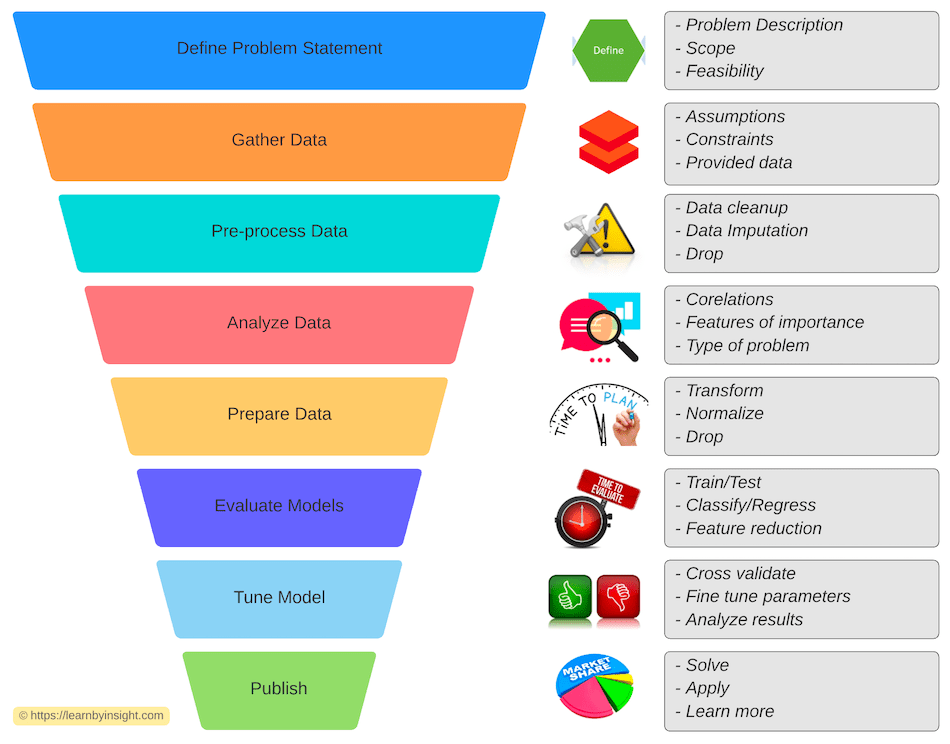
\includegraphics[width=\linewidth]{fig/ml_workflow.png}
    \caption{แนวทางและขั้นตอนการสร้างโมเดลปัญญาประดิษฐ์แบบที่ 1 (เครดิตภาพ: \url{https://learnbyinsight.com})}
    \label{fig:ml_workflow}
\end{figure}

\begin{figure}[htbp]
    \centering
    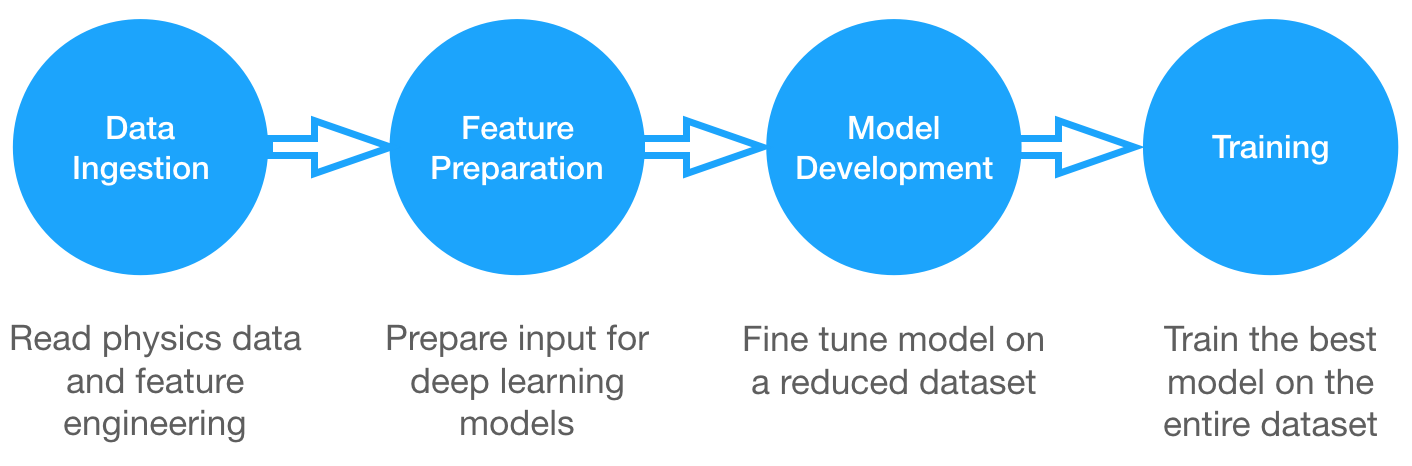
\includegraphics[width=\linewidth]{fig/ml_pipeline.png}
    \caption{แนวทางและขั้นตอนการสร้างโมเดลปัญญาประดิษฐ์แบบที่ 2 (เครดิตภาพ: \url{https://vitalflux.com})}
    \label{fig:ml_pipeline}
\end{figure}

%--------------------------
\section{การเลือกโมเดลที่เหมาะสม}
\label{sec:choose_ml_model}
\idxen{Model Selection}
%--------------------------

\begin{figure}[htbp]
    \centering
    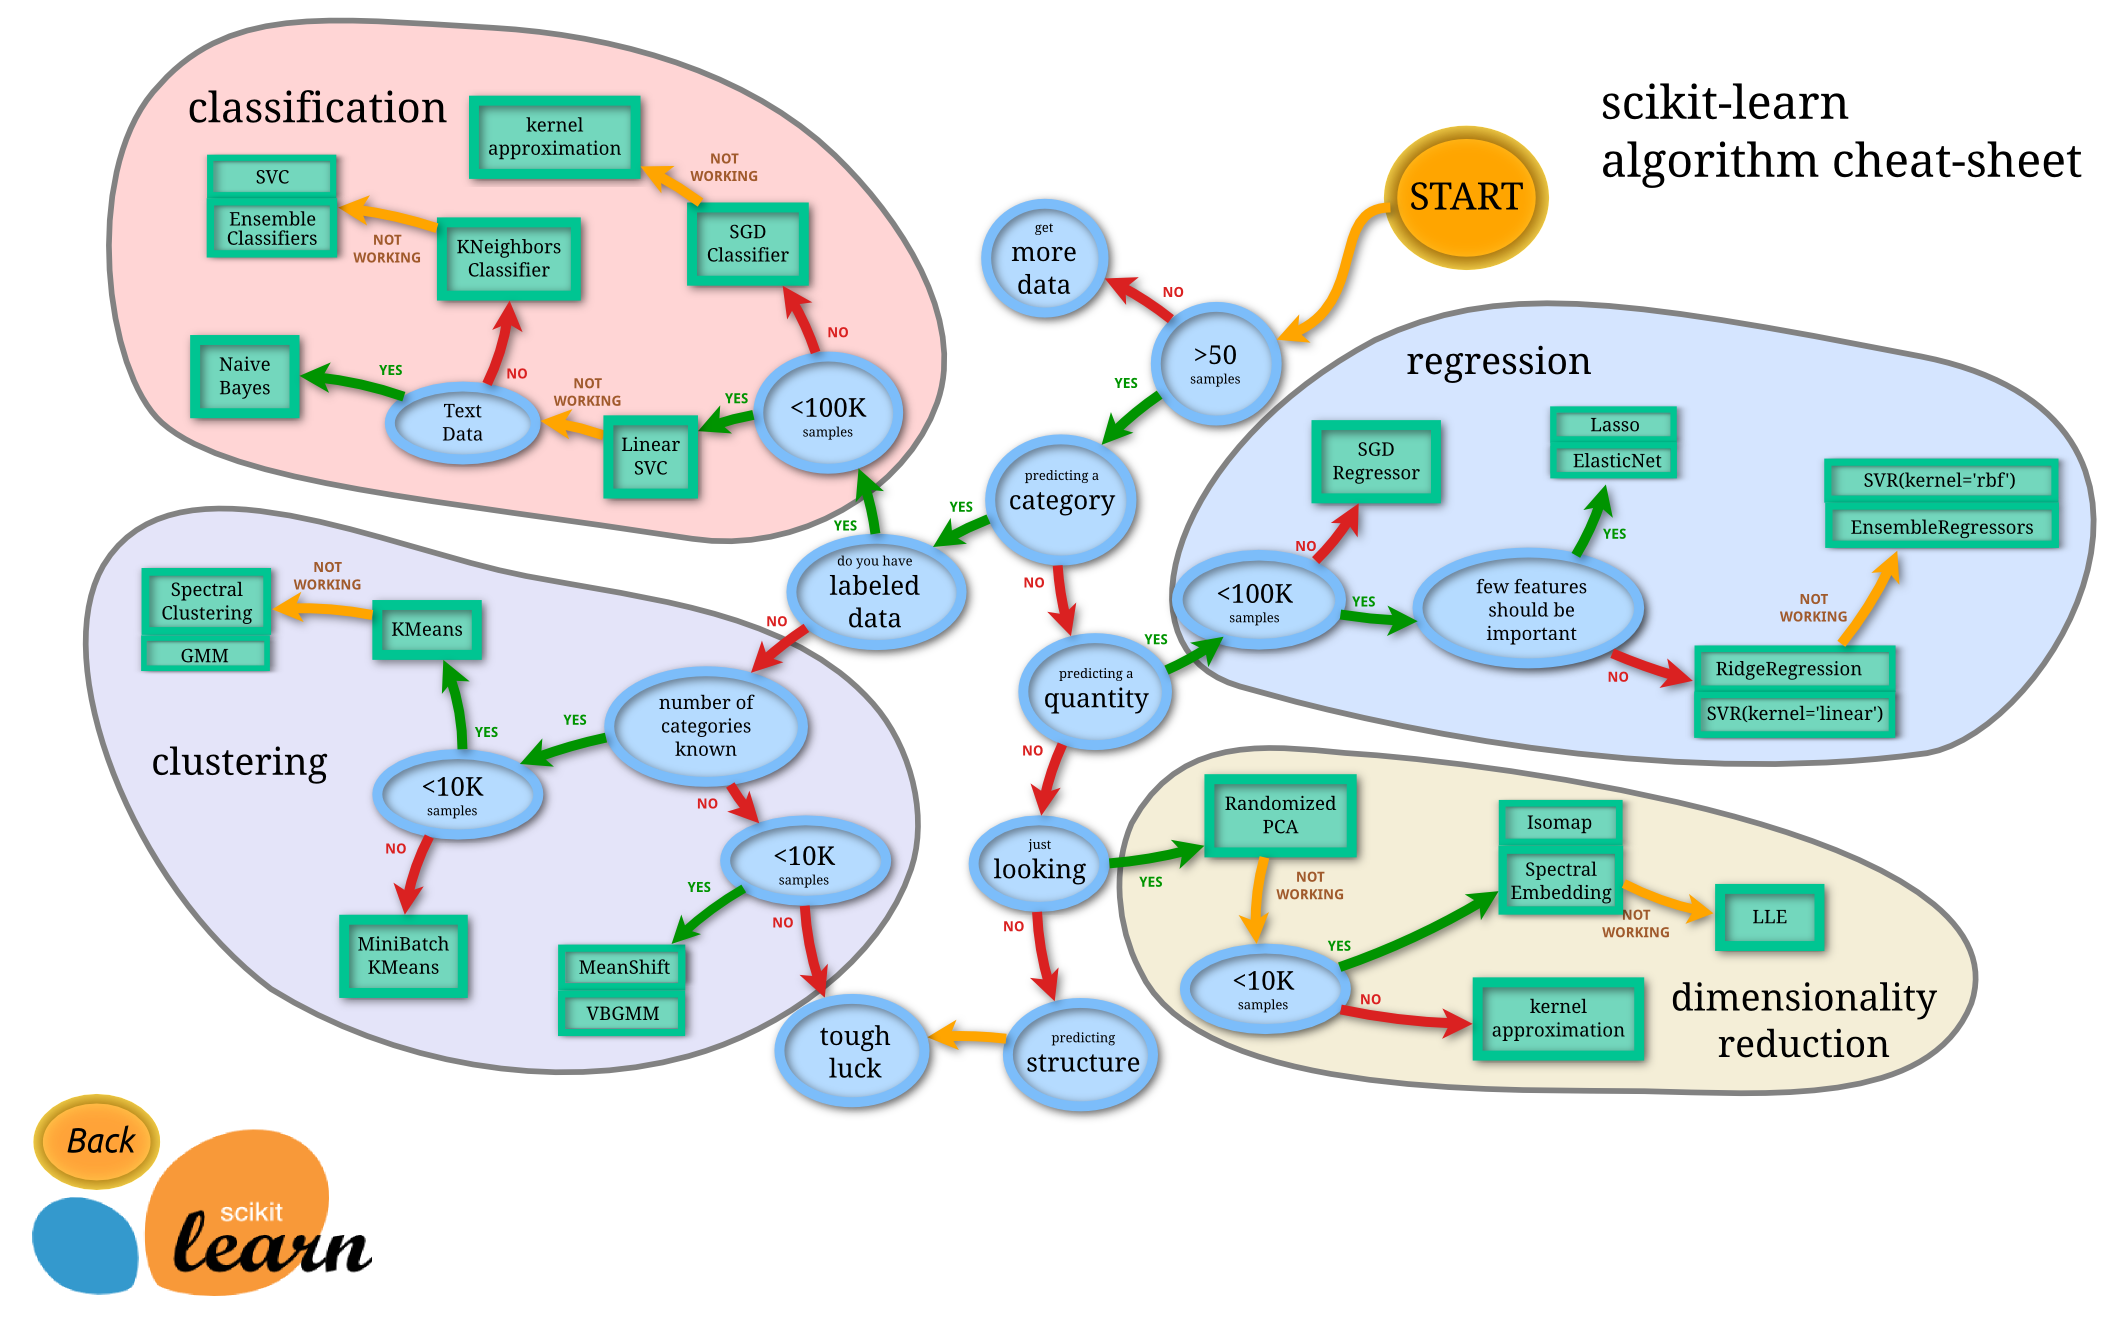
\includegraphics[width=1.3\linewidth,angle=90]{fig/ml_map.png}
    \caption{แผนภาพการเลือกใช้โมเดลปัญญาประดิษฐ์ (เครดิตภาพ: \url{https://scikit-learn.org})}
    \label{fig:ml_map}
\end{figure}

ตัวอย่างของเคอร์เนล (Kernel) ที่มักถูกใช้สำหรับการทำ Regression
\idxboth{เคอร์เนล}{Kernel}

\fbox{%
\begin{minipage}{0.9\linewidth}
    \begin{align*}  
        &\text{Linear Kernel}: &&K(x_i, x_j) = x_i \cdot x_j \\[0.5ex]
        &\text{Polynomial Kernel}: &&K(x_i, x_j; a, b) = (x_i \cdot x_j + a)^b \\[0.5ex]
        &\text{Gaussian Kernel}: &&K(x_i, x_j; w, \sigma) = \mathrm{exp} \left(-\frac{|x_i-x_j|^2}{2\sigma^2} 
        \right) \\[1.5ex]
        &\text{Laplacian Kernel}: &&K(x_i, x_j; w, \gamma) = \mathrm{exp} \left(-{|x_i-x_j|}\right) \\[0.5ex]
    \end{align*}
\end{minipage}}
\idxboth{เคอร์เนล!เชิงเส้น}{Kernel!Linear}
\idxboth{เคอร์เนล!พหุนาม}{Kernel!Polynomial}
\idxboth{เคอร์เนล!เกาส์เซียน}{Kernel!Gaussian}
\idxboth{เคอร์เนล!ลาปลาเซียน}{Kernel!Laplacian}

%--------------------------
\section{การทำนายพลังงานรวมของโมเลกุล}
\label{sec:pred_tot_ener}
\idxth{การทำนายคุณสมบัติของโมเลกุล!พลังงานรวมของโมเลกุล}
\idxen{Molecular Property Prediction!Total Energy}
%--------------------------

การคำนวณพลังงานรวมเชิงอิเล็กทรอนิกส์ของโมเลกุลถือได้ว่าเป็นหนึ่งในการคำนวณพื้นฐานที่สุดในการศึกษาความเสถียรของโมเลกุลเลยก็ว่าได้
โดยเราจะมาดูการเขียนโค้ดสำหรับการทำนายพลังงานของโมเลกุลจากชุดข้อมูล QM9 โดยใช้ Feature ที่เป็น Coulomb Matrix (CM) 
ซึ่งเราได้ดูรายละเอียดการคำนวณ CM รวมถึงการวิเคราะห์ไปแล้วในหัวข้อที่ \ref{sec:dataset_analysis} โดยโมเดล ML ที่ผู้เขียนเลือกคือ
Molecular Kernel สำหรับการทำ Regression ซึ่งสามารถเรียกใช้ได้จากไลบรารี่ QML

ไอเดียของ Molecular Kernel ก็คือเริ่มต้นด้วยการกำหนด Kernel ขึ้นมาก่อน ดังนี้

\begin{equation}\label{eq:mol_kernel}
    \alpha = (\mathbf{K} + \lambda\mathbf{I} ) ^{-1} \mathbf{y}
\end{equation}

\noindent เป้าหมายของเราก็คือการหาค่าของพารามิเตอร์ $\alpha$ ซึ่งเป็นสัมประสิทธิ์ที่เหมาะสมที่สุด (Best Fit for Regression) 
นั่นหมายความว่าเราจะต้องทำการแก้สมการที่ \ref{eq:mol_kernel} ซึ่งสามารถทำได้โดยใช้ Cholesky Decomposition%
\footnote{การแยกส่วนประกอบโชเลสกี (Chlesky Decomposition เป็นวิธีการแยกเมทริกซ์ของเมทริกซ์สมมาตรที่เป็นบวกแน่นอน (Symmetric 
Positive-definite Matrix) ไปเป็นเมทริกซ์สามเหลี่ยมล่าง (Lower Triangular Matrix, $L$) และเมทริกซ์สลับเปลี่ยนของเมทริกซ์สาม%
เหลี่ยมล่าง ($L^{T}$)}

เราเริ่มต้นเขียนโค้ดสำหรับแบ่งชุดข้อมูลออกเป็นชุดข้อมูลสำหรับการฝึกสอนและการทดสอบตามลำดับ
\begin{lstlisting}[style=MyPython]
from sklearn.model_selection import train_test_split

X_cm_train, X_cm_test, Y_cm_train, Y_cm_test = train_test_split(cm, target, test_size=0.2, random_state=42)
\end{lstlisting}

\noindent ตามด้วยการกำหนด Kernel ซึ่งเราจะใช้ Gaussian Kernel 

\begin{equation}\label{eq:gaussian_kernel}
    K(x_{i}, x_{j}) = \mathrm{exp}\left( -\frac{||x_i-x_j||^2}{2\sigma^2} \right)
\end{equation}

\noindent พร้อมกับสร้างลิสต์ของ $\sigma$ หลาย ๆ ค่า ซึ่งเราจะทำการหาค่าที่ดีที่สุดโดยการคำนวณระยะห่างแบบคู่ (Pairwise) ระหว่าง CM 
เพื่อเพิ่มความเร็วในการคำนวณเพราะว่าเราจะทำการแก้ Kernel หลาย ๆ อันพร้อมกับเปลี่ยนค่า $\sigma$ หลาย ๆ ค่าไปพร้อม ๆ กัน

\begin{lstlisting}[style=MyPython]
# Generates a list of different sigma values
sigmas = np.arange(100,5000,500) 
test_maes = []

# Compute the pairwise distances between cm representations
dm_train_train = sklearn.metrics.pairwise_distances(X_cm_train, X_cm_train, n_jobs=-1)
dm_train_test = sklearn.metrics.pairwise_distances(X_cm_train, X_cm_test, n_jobs=-1)
\end{lstlisting}

\noindent หลังจากนั้นจึงเริ่มทำการหาค่า $\sigma$ โดยใช้ Loop

\begin{lstlisting}[style=MyPython]
for sigma in sigmas:
    # Step 1
    K_cm = np.exp( - dm_train_train ** 2 / (2 * sigma ** 2)) 
    # Step 2
    K_cm[np.diag_indices_from(K_cm)] += 1e-8
    # Step 3
    alpha_cm = cho_solve(K_cm, Y_cm_train)
    # Step 4
    K_cm_test = np.exp( - dm_train_test ** 2 / (2 * sigma ** 2))
    # Step 5
    Y_cm_predicted = np.dot(K_cm_test.T, alpha_cm)
    # Step 6
    test_MAE = np.mean(np.abs(Y_cm_predicted - Y_cm_test))
    test_maes.append(test_MAE)
\end{lstlisting}

โดยสิ่งที่เกิดขึ้นภายใน Loop ของโค้ดด้านบนมีดังนี้

\begin{enumerate}[noitemsep]
    \item เราเริ่มด้วยการคำนวณ Kernel ซึ่งถูกกำหนดด้วยสมการ \ref{eq:mol_kernel}
    
    \item เพิ่มค่า $\lambda$ ที่มีค่าน้อย ๆ เข้าไปในสมาชิกแนวทแยงของ Kernel Matrix
    
    \item แก้สมการโดยใช้ Cholesky Decomposition
    
    \item คำนวณ Kernel Matrix ระหว่างชุดข้อมูลที่ใช้ฝึกสอนกับชุดที่ใช้ทดสอบโดยใช้ค่า $\sigma$ เดียวกัน
    
    \item ทำการพยากรณ์หรือทำนายค่าพลังงานภายในของโมเลกุล
    
    \item คำนวณค่าความคลาดเคลื่อน Mean Absolute Error (MAE)
\end{enumerate}

เมื่อทำ Regression เสร็จแล้ว เราสามารถพล็อตกราฟเพื่อดูความสัมพันธ์ค่า $\sigma$ ของ Kernel กับค่าความคลาดเคลื่อน MAE ได้ดังนี้

\begin{lstlisting}[style=MyPython]
import matplotlib.pyplot as plt

fig, ax = plt.subplots()

ax.plot(sigmas, test_maes)
ax.set_ylabel('MAE kcal/mol', fontsize=15)
ax.set_xlabel('Kernel width $\sigma$', fontsize=15)
ax.tick_params(axis='both', which='major', labelsize=12)

plt.show()
\end{lstlisting}

\begin{figure}[htbp]
    \centering
    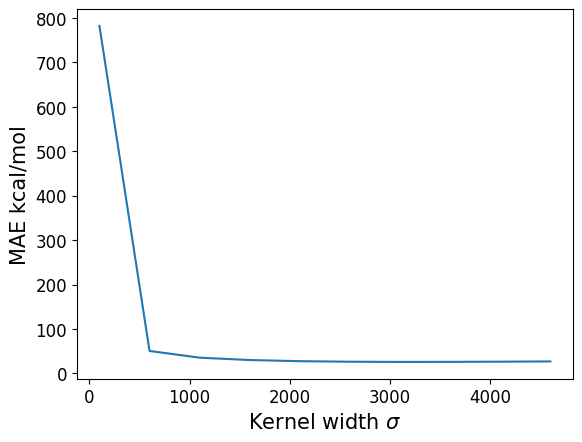
\includegraphics[width=0.9\linewidth]{fig/qm9_cm_mae_sigma.png}
    \caption{ค่าความคลาดเคลื่อน MAE กับค่าความกว้างของ Kernel ($\sigma$)}
    \label{fig:qm9_cm_kernel_mae}
\end{figure}

นอกจากนี้เรายังสามารถทำการวิเคราะห์เพิ่มเติมได้ เช่น แสดงว่า $\sigma$ ที่ดีที่สุด (ให้ MAE น้อยที่สุด)

\begin{lstlisting}[style=MyPython]
best_sigma = sigmas[np.argmin(test_maes)]
print(best_sigma)

# Output
3100
\end{lstlisting}

\noindent แล้วนำค่า $\sigma$ ที่ดีที่สุดนี้ไปใช้สำหรับคำนวณ Gaussian Kernel ต่อได้

\begin{lstlisting}[style=MyPython]
# Create Gaussian Kernel
K_cm = gaussian_kernel(X_cm_train, X_cm_train, sigma)

# Add a small lambda to the diagonal of the kernel matrix
K_cm[np.diag_indices_from(K_cm)] += 1e-8

# Use the built-in Cholesky-decomposition to solve
alpha_cm = cho_solve(K_cm, Y_cm_train)
print(alpha_cm)

# Output
[-1.72214025e+09 -1.37779221e+09 -6.40402006e+08 ...  2.42741968e+09  5.94869282e+08
 -1.19747799e+09]
\end{lstlisting}

\noindent แล้วคำนวณต่อ Kernel ระหว่างชุดข้อมูลฝึกสอนกับชุดข้อมูลทดสอบได้โดยใช้ค่า $\sigma$ เดียวกัน

\begin{lstlisting}[style=MyPython]
# calculate a kernel matrix between test and training data, using the same sigma
K_cm_test = gaussian_kernel(X_cm_test, X_cm_train, sigma)

# Make the predictions
Y_cm_predicted = np.dot(K_cm_test, alpha_cm)

# Calculate mean-absolute-error (MAE), the units are Hartree
print('MAE: ', np.mean(np.abs(Y_cm_predicted - Y_cm_test)), 'kcal/mol')

# Output
MAE:  25.908959327933474 kcal/mol
\end{lstlisting}

ขั้นตอนสุดท้ายคือการพล็อต Correlation ระหว่างค่าอ้างอิง (Reference) กับค่าที่ได้จากการทำนาย (Prediction) และแสดง Histogram 
ของความคลาดเคลื่อนเพื่อตรวจสอบประสิทธิภาพของโมเดล

\begin{lstlisting}[style=MyPython]
import matplotlib.pyplot as plt

fig, axes = plt.subplots(ncols=1, nrows=2, figsize=[6,8])

ax = axes[0]
ax.scatter(Y_cm_test, Y_cm_predicted, s=16)
ax.set_ylabel('CM-KRR internal energies at 0 K \n prediction [kcal/mol]', fontsize=15)
ax.set_xlabel('Internal energies at 0 K [kcal/mol]', fontsize=15)

ax = axes[1]
ax.hist(Y_cm_test - Y_cm_predicted, bins=50, range=[-100,100], density=True)
ax.set_ylabel('Histogram density', fontsize=15)
ax.set_xlabel('CM-KRR internal energies at 0 K errors [kcal/mol]', fontsize=15)

plt.tight_layout()
plt.show()
\end{lstlisting}

\begin{figure}[htbp]
    \centering
    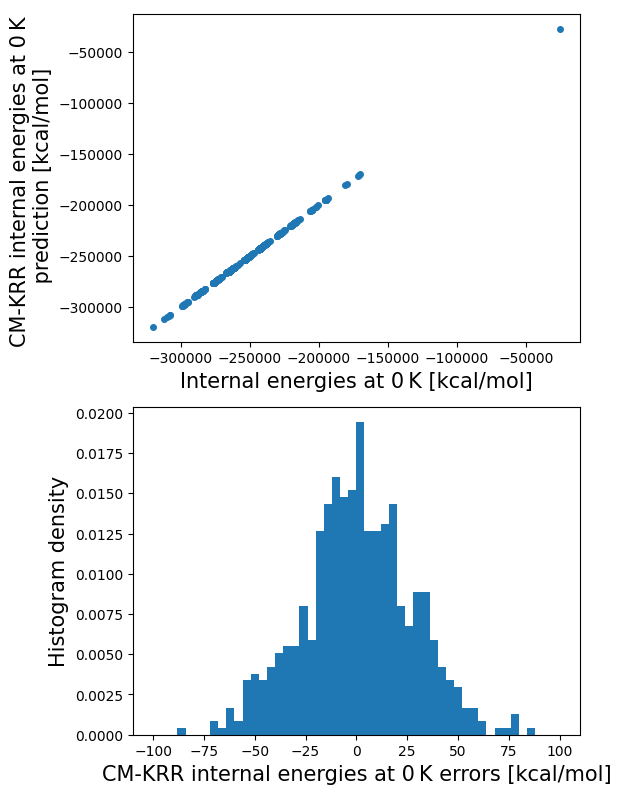
\includegraphics[width=0.8\linewidth]{fig/qm9_cm_kernel_corr.png}
    \caption{ซ้าย: Correlation ของค่าพลังงานภายในของโมเลกุลระหว่างค่าอ้างอิงกับค่าจากการทำนาย, ขวา: Histrogram Density 
    ของค่าคลาดเคลื่อน}
    \label{fig:qm9_cm_kernel_corr}
\end{figure}

%--------------------------
\section{การทำนายพื้นผิวพลังงานศักย์}
\label{sec:pred_pot_ener}
\idxth{การทำนายคุณสมบัติของโมเลกุล!พื้นผิวพลังงานศักย์}
\idxen{Molecular Property Prediction!Potential Energy Surface}
%--------------------------

การทำนายพื้นผิวพลังงานศักย์ (Potential Energy Surface หรือ PES)

Machine Learning Potentials (MLP) เป็นอีกหนึ่งเครื่องมือสำคัญสำหรับการจำลองในระดับอะตอม (Atomistic Simulation) 
โดยเฉพาะการศึกษาพลังงานศักย์ของโมเลกุล\autocite{behler2016,botu2017,brockherde2017,deringer2019,noe2020} 
MLP แบ่งออกได้เป็นสองประเภทตามรูปแบบของอัลกอริทึมของ ML คือ Kernel-based Potentials และ Neural Network-based Potentials

%--------------------------
\subsection{การทำนายพลังงานศักย์ด้วยวิธีเชิงเคอร์เนล}
\label{ssec:pred_pot_ener_kernel}
\idxth{การทำนายคุณสมบัติของโมเลกุล!พื้นผิวพลังงานศักย์!วิธีเชิงเคอร์เนล}
\idxen{Molecular Property Prediction!Potential Energy Surface!Kernel-based}
%--------------------------

เรามาดูรายละเอียดของ Kernel-based Potentials กันก่อน ซึ่งผู้เขียนขอยกมาให้ดู 3 วิธี

\paragraph{Gaussian Approximation Potentials (GAP)} เป็นวิธีที่นำเสนอโดย Albert P. Bart\'{o}k และคณะ ซึ่งตีพิมพ์บทความ%
วิจัยเรื่อง \enquote{Gaussian Approximation Potentials: The Accuracy of Quantum Mechanics, without the Electrons} 
ในวารสาร Physical Review Letters\autocite{bartok2010} GAP เป็นวิธีคำนวณที่ใช้สำหรับการทำนายพลังงานและแรงของแต่ละอะตอม%
ภายในโมเลกุลโดยที่ GAP จะทำการเรียนรู้ค่าทั้งสองจาก PES ซึ่งมักจะได้มาจากการคำนวณด้วยวิธีง่าย ๆ ทั่วไป เช่น DFT 
\idxen{Gaussian Approximation Potentials (GAP)}

GAP นั้นเป็นการทำ Kernel Regression ของ PES แบบ Non-parametric ซึ่งเป็นการประมาณค่าของพลังงานแบบเฉพาะที่ (Local Energy)
ดังนี้

\begin{equation}\label{eq:gap}
    \bar{\epsilon}_{\ast} = \delta^{2} \sum\limits_{s = 1}^{N_s} \alpha_{s} k(\ast,s)
\end{equation}

\noindent โดยที่ $\ast$ หมายถึง Environment ของอะตอมที่เราต้องการทำนาย, $\delta$ คือพารามิเตอร์ที่กำหนดสเกลของพลังงาน, 
$s$ คือจำนวนของ Configuration (ขนาดของ Training Set), $\alpha_{s}$ คือสัมประสิทธิ์ของการ Fitting และ $k(\ast,s)$ 
คือเคอร์เนล

โดยทริคของ GAP คือทำการแปลง PES ที่ปกติจะเป็นฟังก์ชันแบบไม่เป็นเชิงเส้นที่ขึ้นกับตำแหน่งของอะตอม ($E = E(\{ \textbf{r}_i \})$) 
ให้กลายเป็นฟังก์ชันแบบเชิงเส้นที่ขึ้นกับเคอร์เนลแทน พอเรามีฟังก์ชันแบบเชิงเส้นแล้วเราก็สามารถทำ Linear Regression เพื่อหาค่า Parameter 
ต่าง ๆ ที่ใช้ในการ Fit ได้นั่นเอง โดยเคอร์เนลในที่นี้คือการวัดความคล้ายคลึงกันระหว่าง Feature ของอะตอมแต่ละตัวในโมเลกุล (Atomic 
Environment)

\begin{figure}[htbp]
    \centering
    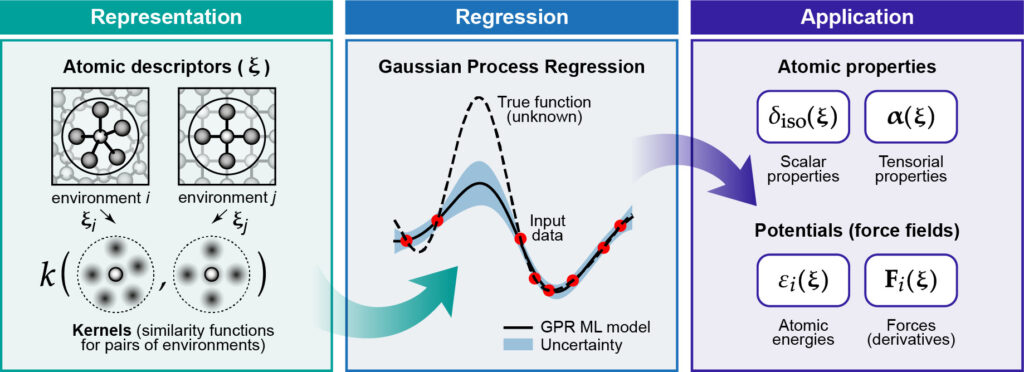
\includegraphics[width=\linewidth]{fig/gap_procedure.jpeg}
    \caption{ขั้นตอนการคำนวณ Representation และการใช้ Gaussian Approximation Potentials ในการทำนายพลังงานและแรง
    (เครดิตภาพ: Deringer และคณะ \textit{Chem. Rev.}, \textbf{2021}, 121, 10073\autocite{deringer2019})}
    \label{fig:gap_procedure}
\end{figure}

ขั้นตอนของการทำ GAP นั้นสามารถดูได้ตามภาพที่ \ref{fig:gap_procedure} โดยมีขั้นตอนดังต่อไปนี้
\begin{enumerate}
    \item เริ่มต้นเราทำการคำนวณหา Representation ก่อนโดยใช้ Atomic Descriptor ซึ่งเป็นข้อมูลหรือ Feature ในระดับอะตอม
    \item หลังจากนั้นทำ Gaussian Process Regression ซึ่งเป็นหัวใจของ GAP
    \item เราจะได้ฟังก์ชันที่สามารถนำไปใช้ในการทำนายพลังงานและแรงเชิงอะตอมได้ ซึ่งสุดท้ายก็สามารถนำมาหาพลังงานรวมของโมเลกุลได้
\end{enumerate}

เนื่องจากว่า GAP ไม่ได้ขึ้นกับฟังก์ชันที่มีรูปแบบตายตัวเหมือนกับ Harmonic Potentials ดังนั้น GAP จึงมีความยืดหยุ่นต่อชุดข้อมูลที่ใช้ในการ%
ฝึกสอน สามารถอธิบายการเปลี่ยนแปลงทางเคมี เช่น การสร้างพันธะหรือการสลายพันธะ ซึ่งเป็นสิ่งที่สนามแรง (Force Field) แบบดั้งเดิมหรือ%
ทั่วไปนั่นทำได้ยาก\autocite{ceriotti2018}

\paragraph{Moment Tensor Potentials (MTP)}
\autocite{shapeev2016}
    
\paragraph{Spectral Neighbor Analysis Potentials (SNAP)} 
\autocite{thompson2015,deng2019,cusentino2020,domina2022}

%--------------------------
\subsection{การทำนายพลังงานศักย์ด้วยวิธีเชิงโครงข่ายประสาท}
\label{ssec:pred_pot_ener_nn}
\idxth{การทำนายคุณสมบัติของโมเลกุล!พื้นผิวพลังงานศักย์!วิธีเชิงโครงข่ายประสาท}
\idxen{Molecular Property Prediction!Potential Energy Surface!Neural Network-based}
%--------------------------

\paragraph{High-dimensional Neural Network Potentials (HDNNP)}
\autocite{behler2007}

\paragraph{ANAKIN-ME} เรียกสั้น ๆ ว่า ANI (ชื่อเต็มคือ Accurate NeurAl networK engINe for Molecular Energies)

\begin{itemize}
    \item ANI-1x\autocite{smith2017}
    \item ANI-1ccx\autocite{smith2018}
    \item ANI-2x\autocite{smith2019,devereux2020}
\end{itemize}

%--------------------------
\section{การจำลองสนามแรง}
\label{sec:model_ff}
\idxth{การทำนายคุณสมบัติของโมเลกุล!สนามแรง}
\idxen{Molecular Property Prediction!Force Field}
%--------------------------

การทำนายหรือพยากรณ์แรง (Forces) และพลังงาน (Energies) ของโมเลกุลนั้นเรียกอีกอย่างหนึ่งว่าการสร้างโมเดล Machine Learning 
Force Field (MLFF) เริ่มต้นสมมติว่าเรามีชุดข้อมูลที่มี Feature Vector ซึ่งเขียนแทนด้วย $\mathbf{D}$ และมีอนุพันธ์แบบเวกเตอร์ 
(Divergence) เป็น $\nabla_{\mathbf{r_i}} \mathbf{D}$ และมีข้อมูลเพิ่มเติมคือพลังงาน $E$ และแรง $\mathbf{F}$ ของระบบ 
(โมเลกุล) สำหรับการฝึกสอนเราจะสร้าง Neural Network (เขียนแทนด้วย $f$) เพื่อสร้างโมเดลสำหรับการทำนายพลังงาน ($\hat{E} = 
f(\mathbf{D})$)\footnote{เครื่องหมาย $\hat{}$\, (อ่านว่า \enquote{hat}) ที่อยู่ด้านบนของตัวแปรเป็นส่งที่บ่งบอกว่าค่าตัวแปรนั้น%
สิ่งที่เราทำนายออกมา} ซึ่งเราสามารถคำนวณแรงได้โดยตรงจากค่าติดลบของ Gradient ของพลังงานเทียบกับพิกัดตำแหน่งของอะตอมนั้น ๆ 
ดังนั้นแรงที่ได้จะเป็นปริมาณต่ออะตอม ยกตัวอย่างเช่นแรงของอะตอม $i$ สามารถคำนวณได้จากสมการต่อไปนี้ (โดยใช้เวกเตอร์แบบแถว)
\idxen{Force Field}

\begin{align}\label{eq:force_pred}
\hat{\mathbf{F}}_i &= - \nabla_{\mathbf{r_i}} f(\mathbf{D}) \\
&= - \nabla_{\mathbf{D}} f \cdot \nabla_{\mathbf{r_i}} \mathbf{D}\\
&= - \begin{bmatrix}
    \frac{\partial f}{\partial D_1} & \frac{\partial f}{\partial D_2} & \dots
\end{bmatrix}
\begin{bmatrix}
    \frac{\partial D_1}{\partial x_i} & \frac{\partial D_1}{\partial y_i} & \frac{\partial D_1}{\partial z_i}\\
    \frac{\partial D_2}{\partial x_i} & \frac{\partial D_2}{\partial y_i} & \frac{\partial D_2}{\partial z_i}\\
    \vdots & \vdots & \vdots \\
\end{bmatrix}
\end{align}

\noindent จากสมการ \ref{eq:force_pred} นั้นเราอธิบายได้ว่า $\nabla_{\mathbf{D}} f$ เป็นค่าอนุพันธ์ของคำตอบของโมเดล ML 
ซึ่งจะเทียบกับ Descriptor $\mathbf{D}$ และ $\nabla_{\mathbf{r_i}} \mathbf{D}$ เป็นอนุพันธ์ของ Descriptor ที่เทียบกับ%
ตำแหน่งของอะตอมซึ่งตามที่เราได้ศึกษามาก่อนหน้านี้ว่า Neural Network นั้นจะให้คำตอบที่เป็นแบบ Analytical Solution

ตัวอย่างของโมเดล ML ที่ถูกพัฒนาขึ้นมาเพื่อเรียนรู้ Force Field ที่น่าสนใจมีดังนี้

\paragraph{FFLUX}\autocite{hughes2019}

\paragraph{TensorMol}\autocite{yao2018}

%--------------------------
\section{การทำนายพลังงานสหสัมพันธ์ของอิเล็กตรอน}
\label{sec:pred_corre_ener}
\idxth{การทำนายคุณสมบัติของโมเลกุล!พลังงานสหสัมพันธ์ของอิเล็กตรอน}
\idxen{Molecular Property Prediction!Correlation Energy}
%--------------------------

\autocite{mcdonagh2018,nudejima2019,dick2020,han2021}

%--------------------------
\section{การทำนายพลังงานกระตุ้นของปฏิกิริยาเคมี}
\label{sec:pred_act_ener}
\idxth{การทำนายคุณสมบัติของโมเลกุล!พลังงานกระตุ้นของปฏิกิริยาเคมี}
\idxen{Molecular Property Prediction!Activation Energy}
%--------------------------

พลังงานกระตุ้น (Activation Energy) เป็นค่าพลังงานที่ต่ำที่สุดที่ใช้เพื่อกระตุ้นปฏิกิริยาเคมี บ่งบอกถึงความยากง่ายของการเกิดปฏิริยาเคมีที่%
สามารถดำเนินไปได้ ณ สภาวะหนึ่ง ๆ ปัจจัยที่มีผลต่อพลังงานกระตุ้น เช่น ความร้อนและตัวเร่งปฏิกิริยา

%--------------------------
\section{การทำนายประจุของอะตอม}
\label{sec:pred_atomic_charge}
\idxth{การทำนายคุณสมบัติของโมเลกุล!ประจุของอะตอม}
\idxen{Molecular Property Prediction!Atomic Charge}
%--------------------------

งานวิจัยทางเคมีควอนตัมที่หัวข้อหนึ่งที่ได้รับความนิยมในช่วง 3-4 ปี (ตั้งแต่ปี ค.ศ. 2018) ที่ผ่านมานี้ที่ได้มีการนำ ML เข้ามาประยุกต์ใช้นั้นก็คือ 
Partial Atomic Charge Assignment หรือการระบุประจุย่อยของอะตอมในโมเลกุล ต้องอธิบายก่อนว่าประจุรวมของโมเลกุลเกิดจากผลรวมของ%
ประจุย่อยของแต่ละอะตอม (Partial Atomic Charge) ซึ่งในทางทฤษฎีและการทดลองเราไม่มีนิยามที่แน่นอนในการระบุหรือกำหนดประจุย่อย%
ของอะตอมแค่ละตัวในโมเลกุล อย่างไรก็ตามได้มีนิยามต่าง ๆ มากมายที่ถูกเสนอขึ้นมาเพื่อใช้ในการ \enquote{คำนวณ} ประจุของแต่ละอะตอม 
โดยแนวคิดแรก ๆ ก็ได้ถูกพัฒนามานานหลายสิบปีแล้ว หนึ่งในนั้นก็คือทฤษฎีที่ตั้งอยู่บนแนวคิดพื้นฐานของ Wavefunction ซึ่งใช้ Population 
ของ Atomic Orbital (Basis Set) เช่น Mulliken Population ที่เราสามารถนำมาใช้ในการคำนวณประจุอะตอม เรียกว่าประจุของมัลลิเคน 
(Mulliken Charge) ซึ่งออร์บิทัลของอะตอมที่อยู่ในโมเลกุลถูกกำหนดและแบ่งด้วยเมทริกซ์ซ้อนทับ (Overlap Matrix) เนื่องจากว่าประจุย่อย%
ของอะตอมเป็นปริมาณที่วัดไม่ได้ (Non-observable Property) ซึ่งไม่สามารถวัดได้ในทางทดลอง นั่นก็เพราะว่าจริง ๆ แล้วไม่มีอะตอมในโมเลกุล 
มีแต่กลุ่มก้อนของอิเล็กตรอน ดังนั้นเราจึงไม่สามารถที่จะระบุได้ว่าอะตอมแต่ละตัวนั้นมีขนาดเล็กหรือใหญ่แค่ไหน กล่าวคือเราไม่รู้ว่าอะตอมและตัวเริ่มต้น%
ตรงไหนและสิ้นสุดตรงไหน นั่นจึงทำให้เราไม่รู้ขอบเขตของแต่ละอะตอมนั่นเอง

นอกจากนี้ยังมีอีกหลายทฤษฎี/วิธีที่ได้ถูกพัฒนาขึ้นมาเพื่อกำหนดนิยามของประจุย่อยของอะตอม ดังนี้

\begin{enumerate}
    \item วิธีที่ใช้ออร์บิทัล (Orbital-based) ซึ่งเป็นการทำ Population โดยใช้ Basis Functions
        \begin{enumerate}
            \item Mulliken Charge\autocite{szabo1996}
            
            \item L\"{o}wdin Charge\autocite{lowdin1950}
        \end{enumerate}
    
    \item วิธีที่ใช้ศักย์เชิงไฟฟ้าสถิตย์ (Electrostatic Potential-based)
        \begin{enumerate}
            \item Merz-Kollman Charge\autocite{singh1984}
            
            \item Charges from the Electrostatic Potential (CHELP) Charge\autocite{chirlian1987}
            
            \item Charges from the Electrostatic Potential on a Grid (CHELPG) Charge\autocite{breneman1990}
            
            \item Restrained Electrostatic Potential (RESP)\autocite{cornell1993}
        \end{enumerate}
    
    \item วิธีที่ใช้ความหนาแน่นของอิเล็กตรอน (Electron Density-based)
    \begin{enumerate}
        \item Hirshfeld Charge\autocite{hirshfeld1977}
        
        \item Atoms in Molecules (AIM) หรือ Bader Charge\autocite{bader1985,bader1991}
    \end{enumerate}
    
    \item เทนเซอร์เชิงขั้ว (Polar Tensor)\autocite{person1974,milani2010}
        \begin{enumerate}
        \item Atomic Polar Tensor (APT) Charge \\
        $q_{i} = \frac{1}{3}\Big(\pdv{\mu_{x}}{x_{i}} + \pdv{\mu_{y}}{y_{i}} + \pdv{\mu_{z}}{z_{i}}\Big)$
        \end{enumerate}
\end{enumerate}

งานวิจัยโดดเด่นและได้รับการตีพิมพ์ในวารสารชั้นแนวหน้าที่ใช้ ML เข้ามาในการทำนายหรือระบุประจุของอะตอม ที่ผู้เขียนได้เลือกมาซึ่งเรียงลำดับตาม 
Timeline มีดังนี้

\begin{itemize}
    \item \enquote{Fast and Accurate Generation of \textit{ab initio} Quality Atomic Charges Using Nonparametric 
    Statistical Regression}\autocite{rai2013} \\ 
    หนึ่งในงานวิจัยแรก ๆ ที่เริ่มมีการประยุกต์เทคนิคทางสถิติ (Regression) เข้ามาใช้ในการสร้างโมเดลเรียนรู้การทำนายประจุย่อย
    
    \item \enquote{Machine Learning of Partial Charges Derived from High-Quality Quantum-Mechanical Calculations} 
    \autocite{bleiziffer2018} \\
    งานวิจัยที่ต่อยอดมาจากงานของ โดยใช้ Feature ที่ชื่อว่า \enquote{Atom-centered Atom-pairs Fingerprint}\autocite{carhart1985} 
    ในการฝึกสอนโมเดลและนำมาใช้ในทำนายประจุย่อยได้อย่างแม่นยำมาก ๆ
    
    \item \enquote{Transferable Dynamic Molecular Charge Assignment Using Deep Neural Networks}\autocite{nebgen2018} \\
    งานวิจัยนี้ใช้ Neural Network ในการทำนายประจุย่อยแบบไดนามิกส์
    
    \item \enquote{PhysNet: A Neural Network for Predicting Energies, Forces, Dipole Moments, and Partial Charges}
    \autocite{unke2019} \\
    งานวิจัยนี้นำเสนอโมเดล ML ที่ชื่อว่า PhysNet ซึ่งสามารถทำนายคุณสมบัติเชิงโมเลกุล ประกอบไปด้วย พลังงาน, แรง, ไดโพล โมเมนต์, 
    และประจุย่อย
    
    \item \enquote{Fast and Accurate Machine Learning Strategy for Calculating Partial Atomic Charges in 
    Metal-Organic Frameworks}\autocite{kancharlapalli2021} \\ 
    งานวิจัยนี้เป็นการทำนายประจุของอะตอมในสารประกอบ Metal-Organic Frameworks (MOFs)
    
    \item \enquote{High-Precision Atomic Charge Prediction for Protein Systems Using Fragment Molecular Orbital 
    Calculation and Machine Learning}\autocite{kato2020} \\ 
    งานวิจัยนี้สนใจการทำนายประจุเชิงอะตอมของโปรตีโดยใช้ Fragment Molecular Orbital
    
    \item \enquote{DeepChargePredictor: A Web Server for Predicting QM-based Atomic Charges via State-of-the-art 
    Machine-learning Algorithms}\autocite{wang2021} \\ 
    งานวิจัยนี้พัฒนาเว็บไซต์ที่ช่วยให้เราสามารถทำนายประจุย่อยได้
\end{itemize}

%--------------------------
\section{การทำนายไดโพลโมเมนต์}
\label{sec:pred_dipole_moment}
\idxth{การทำนายคุณสมบัติของโมเลกุล!การทำนายไดโพลโมเมนต์}
\idxen{Molecular Property Prediction!Dipole Moment}
%--------------------------

%--------------------------
\section{การทำนายคุณสมบัติของโมเลกุลที่สภาวะกระตุ้น}
\label{sec:pred_ex_prop}
\idxth{การทำนายคุณสมบัติของโมเลกุล!คุณสมบัติของโมเลกุลที่สภาวะกระตุ้น}
\idxen{Molecular Property Prediction!Excited State}
%--------------------------

หนึ่งในงานวิจัยที่น่าสนใจที่ตีพิมพ์ในบทความ \enquote{Excited State Non-adiabatic Dynamics of Large Photoswitchable Molecules 
Using a Chemically Transferable Machine Learning Potential}\autocite{axelrod2022} มีงานวิจัยที่ได้ใช้ ML ในการทำนาย 
Quantum Yield\footnote{ผู้เขียนขอใช้ทับศัพท์เพราะถ้าหากช้คำแปลเป็นภาษาไทยจะใช้คำว่า \enquote{ผลผลิตควอนตัม} ซึ่งยากต่อการเข้าใจ 
ดังนั้นจึงขอใช้คำว่า Quantum Yield ตรง ๆ} ของโมเลกุลขนาดใหญ่ ณ สภาวะกระตุ้น ซึ่งในงานวิจัยนี้ได้ศึกษาอนุพันธ์ของโมเลกุลเอโซเบนซีน 
(Azobenzene) รวมถึงไปการทรานซิชันระหว่างคอนฟอร์เมอร์ \textit{cis} กับ \textit{trans} อีกด้วย

%--------------------------
\section{การทำนายค่าคู่ควบเชิงเล็กอิเล็กทรอนิกส์}
\label{sec:pred_elec_coupling}
\idxth{การทำนายคุณสมบัติของโมเลกุล!ค่าคู่ควบเชิงเล็กอิเล็กทรอนิกส์}
\idxen{Molecular Property Prediction!Electronic Coupling}
%--------------------------

ค่าคู่ควบเชิงเล็กอิเล็กทรอนิกส์ (Electronic Coupling) คือค่าความเกี่ยวเนื่องเชิงอิเล็กทรอนิกส์ระหว่าง 2 สถานะใด ๆ ของอิเล็กตรอน เช่น 
สถานะเริ่มต้นและสถานะสิ้นสุดในกระบวนการทางควอนตัม 

%--------------------------
\subsection{ค่าคู่ควบของการถ่ายโอนอิเล็กตรอน}
\label{ssec:pred_etran_coupling}
\idxth{การทำนายคุณสมบัติของโมเลกุล!ค่าคู่ควบของการถ่ายโอนอิเล็กตรอน}
\idxen{Molecular Property Prediction!Electron Transfer Coupling}
%--------------------------



%--------------------------
\subsection{ค่าคู่ควบแบบนอนอะเดียแบติก}
\label{ssec:nonadia_coupling}
\idxth{การทำนายคุณสมบัติของโมเลกุล!ค่าคู่ควบแบบนอนอะเดียแบติก}
\idxen{Molecular Property Prediction!Nonadiabatic Coupling}
%--------------------------



%--------------------------
\section{การทำนายสเปกตรัม}
\label{sec:pred_spectra}
\idxth{การทำนายคุณสมบัติของโมเลกุล!การทำนายสเปกตรัม}
\idxen{Molecular Property Prediction!Spectra}
%--------------------------

การทำนายสเปกตรัมเป็นอีกหนึ่งหัวข้องานวิจัยทางด้านเคมีควอนตัมที่ได้รับความสนใจเป็นอย่างมากนั่นก็เพราะว่าเทคนิคทางสเปกโทรสโกปีนั้นมีประโยชน์%
อย่างมากในงานทางด้านเคมีสังเคราะห์ ทั้งเคมีอินทรีย์และเคมีอนินทรีย์ รวมไปถึงด้านอื่น ๆ เช่น วัสดุศาสตร์หรือพอลิเมอร์ด้วย 

สเปกโทรสโกปีเป็นเทคนิคที่เกี่ยวข้องกับแสงซึ่งเป็นคลื่นแม่เหล็กไฟฟ้าที่มีลักษณะเป็นแถบพลังงาน (Spectrum) โดยมีความยาวคลื่นตั้งแต่ในช่วง 
คลื่นวิทยุ คลื่นไมโครเวฟ คลื่นอินฟราเรด คลื่นในช่วงที่สายตามองเห็น รวมถึงคลื่นอัลตราไวโอเลต สำหรับคลื่นแม่เหล็กไฟฟ้าที่นักเคมีสนใจนั้นจะ%
เกี่ยวข้องโดยตรงกับการระบุถึงความจำเพาะเจาะจงของโมเลกุล นั่นคือคลื่นแม่เหล็กไฟฟ้าในช่วงอินฟราเรด ซึ่งจะมีความยาวคลื่น (Wavelength) 
ในช่วง 650 - 4,000 nm หรือมีเลขคลื่น (Wavenumber) ในช่วง 14,286-12,800 $cm^{-1}$ โดยหลักการคร่าว ๆ ของเทคนิคอินฟราเรด%
สเปกโทรโกปีก็คือแสงอินฟราเรดตกกระทบโมเลกุลจะเกิดอันตรกิริยาระหว่างแสงกับโมเลกุล โดยที่แสงอินฟราเรดในบางช่วงที่มีความถี่ตรงกันกับความถี่%
ของการสั่นของพันธะในโมเลกุลจะถูกดูดกลืนไป ซึ่งทำให้เกิดทรานซิชันการสั่นพร้อมกับทรานซิชันการหมุน ซึ่งทรานซิชันการสั่นนี้จะเราทราบชนิดของ%
หมู่ฟังก์ชัน เช่น พันธะคู่ พันธะสาม หมู่คาร์บอนิล หมู่ไฮดรอกซิล หรือหมู่อะมิโน ภายในโครงสร้างของโมเลกุลอินทรีย์ได้ ดังนั้นความเข้มของแสง%
อินฟราเรดที่ทะลุผ่านสารตัวอย่าง (Transmitted Infrared) จึงมีความเข้มแสงลดลงในบางช่วงของความถี่ทั้งหมดของอินฟราเรดเนื่องมาจากการ%
ถูกดูดกลืนโดยหมู่ฟังก์ชันดังกล่าวนั่นเอง

%--------------------------
\subsection{การทำนายอินฟราเรดสเปกโทรโกปี}
\label{ssec:pred_spec_ir}
\idxth{การทำนายคุณสมบัติของโมเลกุล!การทำนายสเปกตรัม!อินฟราเรดสเปกโทรโกปี}
\idxen{Molecular Property Prediction!Spectra!Infrared}
%--------------------------

การทำนายสเปกตรัมอินฟราเรดด้วย ML นั้นได้รับการค้นคว้ามาอย่างต่อเนื่องเป็นระยะเวลาหลายสิบปี\autocite{gastegger2017} สำหรับงานวิจัย%
ที่ผู้เขียนจะยกมาเป็นกรณีศึกษานั้นเป็นงานวิจัยที่มีชื่อบทความว่า \enquote{Infrared Spectra at Coupled Cluster Accuracy from Neural 
Network Representations} หรือแปลเป็นภาษาไทยคือ \enquote{การทำนาย IR Spectrum ที่ระดับความแม่นยำเดียวกับระเบียบวิธี CCSD(T) 
ด้วย Neural Network}\autocite{beckmann2022} โดยงานวิจัยนี้ได้รับการตีพิมพ์ในวารสาร Journal of Chemical Theory and Computation 
(JCTC) ซึ่งเป็นวารสารวิชาการแนวหน้าทางด้านเคมีทฤษฎีและการคำนวณทางคอมพิวเตอร์ 

รายละเอียดงานวิจัยในบทความฉบับนี้มีดังนี้ ผู้วิจัยได้สร้าง Neural Network โดยใช้สถาปัตยกรรมโครงสร้างประสาทของ Behler-Parrinello 
Neural Network (BPNN)\autocite{behler2007,behler2011b,behler2015} ซึ่งเป็น Neural Network เชิงโมเลกุลแบบที่มีมิติมาก 
(High-dimensional Molecular Neural Network) ที่มีแนวคิดคือผลรวมของพลังงานทั้งหมดของโมเลกุลเกิดขึ้นจากการรวมกันของพลังงาน%
ของแต่ละอะตอม โดยที่ Neural Network ที่ผู้วิจัยได้พัฒนาขึ้นมาได้ถูกนำไปใช้ในการเรียนรู้ (Learn) โครงสร้างของโมเลกุลและ Fit เข้ากับค่า 
Dipole Moment ($\mu$) ของโมเลกุลนั้น ๆ ซึ่ง $\mu$ คือพารามิเตอร์สำคัญที่เราสามารถนำไปใช้ในการคำนวณหาความเข้มหรือ Intensity 
ของ IR Spectrum (สำหรับแต่ละ Peak) ต่อไปได้

แต่ว่าผู้วิจัยไม่ได้ Fit ข้อมูลเชิงโครงสร้างของโมเลกุลเข้ากับ $\mu$ โดยตรงเพราะว่าพารามิเตอร์ทั้งสองนี้ไม่ได้สอดคล้องหรือเกี่ยวข้องกันโดยตรง 
ดังนั้นเราควรจะต้องทำการ Fit เข้ากับบางสิ่งบางอย่างที่อธิบายเคมีเชิงอิเล็กทรอนิกของโมเลกุลได้ดีกว่าข้อมูลเชิงโครงสร้างทั่วไป ซึ่งสิ่งนั้นเรียกว่า 
Electronic-based Descriptor โดย Descriptor ที่ผู้วิจัยเลือกใช้ก็คือ Atomic-centered Symmetry Function (ACSF) โดยได้ทำการ 
Fit ACSF เข้ากับประจุย่อยของแต่ละอะตอม (Atomic Partial Charge) ซึ่งผู้อ่านอาจจะสงสัยว่าทำไมถึงไม่ Fit ACSF กับ $\mu$ โดยตรงเลย? 
เหตุผลก็เพราะว่า $\mu$ นั้นถูกคำนวณมาจากผลรวมของผลคูณระหว่างประจุ ($q_{i}$) และตำแหน่งของแต่ละอะตอม ($\vec{r}_{i}$) 
ภายในโมเลกุลตามสมการที่ \ref{eq:dipole_moment}

\begin{equation}\label{eq:dipole_moment}
    \mu = \sum^{N}_{i} q_{i}\vec{r}_{i}
\end{equation}

\noindent ดังนั้นจึงจะเหมาะกว่าถ้าเรา Fit เข้ากับประจุก่อน หลังจากนั้นเอาต์พุตสุดท้ายที่ถูกทำนายออกมาจาก Neural Network นั้นก็จะเป็น 
$\mu$ นั่นเอง สรุปลำดับการ Fit ข้อมูลมีดังนี้ 

\fbox{%
\begin{minipage}[c][1cm]{0.9\linewidth}
\centering
Structure $\rightarrow$ ACSF $\rightarrow$ Atomic Partial Chage $\rightarrow$ Dipole Moment 
\end{minipage}}

นอกจากนี้ผู้วิจัยเลือกใช้ RMSE เป็น Lost Function สำหรับการปรับลด Error ระหว่าง $\mu$ ที่ได้จากการทำนายกับค่าอ้างอิงที่ได้จากการ%
คำนวณด้วยวิธี CCSD(T) โดยใช้โปรแกรม Molpro และได้มีการปรับแต่ง Loss Function โดยทำการคำนวณ Error ของทุกคอนฟอร์เมอร์ 
ซึ่งจะทำการปรับค่าลดค่าคลาดเคลื่อนจาก $\mu$ ของทั้งสามทิศทาง (3 Components) นั่นคือ $x$, $y$ และ $z$ ตามสมการดังต่อไปนี้

\begin{equation}
    \mathcal{L} = \frac{1}{3M} \sum^{M}_{i} \sum^{3}_{\alpha} (\mu^{\text{NN}}_{i,\alpha} 
    - \mu^{\text{ref}}_{i,\alpha})^{2}
\end{equation}

\noindent โดยที่ $M$ คือจำนวนคอนฟอร์เมอร์ และ $\alpha$ คือทิศทาง หลังจากนั้นผู้วิจัยใช้ Autocorrelation Function ในการแปลง 
$\mu$ (เปลี่ยนจาก Time-domain ไปเป็น Frequency-domain) เพื่อคำนวณหาสเปกตรัมของอินฟราเรดต่อไป 

สำหรับชุดโมเลกุลที่ผู้วิจัยศึกษาในงานนี้เป็นแค่กลุ่มโมเลกุลง่าย ๆ คือกลุ่มโมเลกุลน้ำ (Water Cluster) โดยมีการศึกษาความสามารถในการ%
เรียนรู้ของโมเดลที่เปลี่ยนแปลงไปตามขนาดของชุดข้อมูลฝึกสอนและชุดข้อมูลทดสอบ โดยผู้วิจัยได้มีการใช้ชุดข้อมูลฝึกสอนขนาดเล็กสุดคือ 5,975 
โครงสร้างและใหญ่สุดคือ 18,576 โครงสร้าง ซึ่งประสิทธิภาพในการทำนายถือว่าอยู่ในระดับที่แม่นยำมาก โดยมีค่าคลาดเคลื่อนการทำนาย $\mu$ 
ต่อโมเลกุลอยู่ที่ 0.007 D และต่ออะตอมอยู่ที่ประมาณ 0.002 D

%--------------------------
\subsection{การทำนายรามานสเปกโทรโกปี}
\label{ssec:pred_spec_raman}
\idxth{การทำนายคุณสมบัติของโมเลกุล!การทำนายสเปกตรัม!รามานสเปกโทรโกปี}
\idxen{Molecular Property Prediction!Spectra!Raman}
%--------------------------


%--------------------------
\subsection{วิธีการทำนายสเปกตรัมและโครงสร้าง}
\label{ssec:pred_spec_struct}
\idxth{การทำนายคุณสมบัติของโมเลกุล!การทำนายสเปกตรัม!วิธีการทำนายสเปกตรัมและโครงสร้าง}
\idxen{Molecular Property Prediction!Spectra!Predicting Spectra and Structures}
%--------------------------

\begin{table}[H]
    \centering
    \caption{บทความงานวิจัยที่เกี่ยวข้องกับวิธี Struc-to-Spec}
    \label{tab:struc2spec}
    \small
    \begin{tabular}{clll}
    \toprule
    \textbf{Ref.} &\textbf{Learning Target} &\textbf{โมเดล ML} &\textbf{Representation} \\
    \midrule
    \autocite{schuur1996,Schuur1997} & ความเข้มการดูดกลืน IR & PCA+CPG\autocite{hecht-nielsen1987}, 
    CPG\autocite{hecht-nielsen1987} & คุณสมบัติเชิงอะตอม, ระยะห่างระหว่างอะตอม \\
    
    \autocite{selzer2000,kostka2001} & ความเข้มการดูดกลืน IR & \makecell[tl]{Query Driven Selection \\ + RDF + 
    CPG\autocite{hecht-nielsen1987}} & คุณสมบัติเชิงอะตอม, ระยะห่างระหว่างอะตอม \\
    
    \autocite{yildiz2011,yildiz2012} & ความเข้ม IR/Raman & LFFN-EPFs\autocite{yildiz2011} & ความเข้ม IR/Raman \\
    
    \autocite{gastegger2017} & ประจุย่อยเชิงอะตอม & HDNNP\autocite{behler2007} + ED-GEKF\autocite{gastegger2015} 
    & ACSFs\autocite{behler2011a}, Geometric Descriptors \\
    
    \autocite{sifain2018,nebgen2018} & ประจุย่อยเชิงอะตอม & HIP-NN\autocite{lubbers2018} & เลขอะตอม, 
    ระยะห่างระหว่างอะตอม \\
   \bottomrule
\end{tabular}
\end{table}

\begin{table}[H]
    \centering
    \caption{บทความงานวิจัยที่เกี่ยวข้องกับวิธี Spec-to-Struc}
    \label{tab:spec2struc}
    \small
    \begin{tabular}{clll}
    \toprule
    \textbf{Ref.} &\textbf{Learning Target} &\textbf{โมเดล ML} &\textbf{Representation} \\
    \midrule
    \autocite{visser1994,luinge1995} & โครงสร้างและหมู่ฟังก์ชัน & 
    PLS\autocite{wold1984}, PCA-MLP, MLP & \makecell[tl]{Band Pattern \\ Full Spectrum} \\

    \autocite{carrieri1995} & โมเลกุลทั่วไป & Binary และ Decimal-based NN & 
    Band Pattern \\
    
    \autocite{fu2018} & คอนฟิกูเรชั่นเชิงนิวเคลียร์ & Basin-hopping Algorithm\autocite{wales1997} & 
    Cosine Distances \\
    
    \autocite{fine2020} & หมู่ฟังก์ชัน & Autoencoder + MLP, RF\autocite{breiman2001} & 
    Peak ของ FTIR \\
    
    \autocite{ren2021} & โครงสร้างที่มีหมู่ \ce{OH} และ \ce{C=O} & LSTM \autocite{hochreiter1997} & 
    \makecell[tl]{Peak ของ IR และ Raman \\ ที่คำนวณด้วย DFT} \\
   \bottomrule
\end{tabular}
\end{table}

\begin{itemize}[topsep=0pt,noitemsep]
    \item CPG: Counterpropagation
    
    \item ED-GEKF: Element-decoupled Global Extended Kalman Filter
    
    \item FTIR: Fourier Transform Infrared
    
    \item HDNNP: High Dimensional Neural Network Potential
    
    \item HIP-NN: Hierarchically Interacting Particle Neural Network
    
    \item LFFN-EPFs: Layered Feed Forward Neural Network - Empirical Physical Formulas
    
    \item MLP: Multilayer Perceptron
    
    \item NMA: N-methylacetamide
    
    \item PCA: Principal Component Analysis
    
    \item PG-EA: Probability Graph-evolutionary Algorithm
    
    \item RDF: Radial Distribution Function
\end{itemize}

\idxen{Molecular Property Prediction!Spectra!Struc-to-Spec}
\idxen{Molecular Property Prediction!Spectra!Spec-to-Struc}

%--------------------------
\section{บทความวิชาการเพิ่มเติม}
\label{sec:pred_misc_papers}
%--------------------------

นอกเหนือจากการนำ ML ไปใช้สำหรับการทำนายพารามิเตอร์ต่าง ๆ แล้ว ถ้าหากผู้อ่านสนใจการประยุกต์ใช้ ML กับงานทางด้านอื่น ๆ ของเคมีควอนตัม 
สามารถอ่านบทความวิชาการเพิ่มเติมได้จากวารสารวิชาการชั้นแนวหน้า เช่น 

\begin{itemize}[topsep=0pt,noitemsep]
    \item Journal of Chemical Information and Modeling (\textit{J. Chem. Inf. Model}) 
    
    \item Journal of Chemical Physics (\textit{J. Chem. Phys.}) 
    
    \item Journal of Chemical Theory and Computation (\textit{J. Chem. Theory Comput.}) 
    
    \item Journal of Physical Chemistry A (\textit{J. Phys. Chem. A}) 
    
    \item Journal of Physical Chemistry Letters (\textit{J. Phys. Chem. Lett.}) 
    
    \item Machine Learning: Science and Technology (\textit{MLST}) 
    
    \item Nature Machine Intelligence (\textit{Nat. Mach. Intell}) 
    
    \item Nature Communications (\textit{Nat. Commun.})
    
    \item Proceedings of the National Academy of Sciences of the United States of America (\textit{PNAS}) 
    
    \item Science Advances (\textit{Sci. Adv.}) 
\end{itemize}

\noindent โดยวารสารอันดับที่ 1-5 เป็นวารสารเฉพาะทางด้านเคมีทฤษฎีและเคมีคอมพิวเตอร์, วารสารอันดับที่ 6-7 เป็นวารสารเฉพาะทางด้าน%
การเรียนรู้ของเครื่อง, และวารสารอันดับที่ 8-10 เป็นวารสารด้านวิทยาศาสตร์ทั่วไป นอกจากนี้แล้วยังมีวารสารอื่น ๆ อีกที่ไม่ได้กล่าวถึงรวมไปถึง
Repository ที่ให้บริการเผยแพร่บทความงานวิจัยแบบเข้าถึงได้ฟรี (Open-access) เช่น arXiv และ ChemRxiv

%--------------------------
\subsection{บทความเฉพาะทาง}
\label{ssec:pred_misc_papers_specific}
%--------------------------

โดยผู้เขียนได้เลือกงานวิจัยที่มีความโดดเด่นและเหมาะสำหรับผู้เริ่มต้นศึกษา ML และเคมีควอนตัม ซึ่งน่าจะช่วยให้ผู้อ่านเห็นภาพรวมของโจทย์งานวิจัย%
ในปัจจุบันที่กำลังมาแรง บทความที่คัดเลือกมาประกอบไปด้วยบทความการทบทวนงานวิจัย (Review) ที่ใช้ ML ในการเรียนรู้ Force Field 
สำหรับงานทางด้านเคมีควอนตัมและการจําลองพลวัตเชิงโมเลกุล (QM/MD) หรือนำมาใช้ในการทำนายพื้นที่พลังงานอิสระ (Free Energy Landscape)
ไปจนถึงการพัฒนาโมเดล ML เพื่อทำนายคุณสมบัติเชิงโมเลกุล เช่น ไดโพลโมเมนต์ (Dipole Moment) และสภาพการเกิดขึ้น (Polarizability)

\begin{enumerate}
    \item \enquote{PhysNet: A Neural Network for Predicting Energies, Forces, Dipole Moments, and 
    Partial Charges}\autocite{unke2019}\\
    ตีพิมพ์เมื่อวันที่ 01 พฤษภาคม ค.ศ. 2019
    
    \item \enquote{Comparison of the Performance of Machine Learning Models in Representing High-Dimensional 
    Free Energy Surfaces and Generating Observables}\autocite{cendagorta2020}\\
    ตีพิมพ์เมื่อวันที่ 10 เมษายน ค.ศ. 2020
    
    \item \enquote{Kernel-Based Machine Learning for Efficient Simulations of Molecular Liquids}\autocite{scherer2020}\\
    ตีพิมพ์เมื่อวันที่ 13 เมษายน ค.ศ. 2020

    \item \enquote{Machine Learning Force Fields}\autocite{unke2021}\\
    ตีพิมพ์เมื่อวันที่ 11 มีนาคม ค.ศ. 2021

    \item \enquote{The Rise of Neural Networks for Materials and Chemical Dynamics}\autocite{kulichenko2021}\\
    ตีพิมพ์เมื่อวันที่ 1 กรกฎาคม ค.ศ. 2021

\end{enumerate}

%--------------------------
\subsection{บทความรีวิว}
\label{ssec:pred_misc_papers_review}
%--------------------------

ในช่วง 5 ปีที่ผ่านมานี้ (ค.ศ. 2017-2022) นอกจากจะมีการตีพิมพ์บทความงานวิจัยเฉพาะทางออกมาอย่างต่อเนื่องแล้ว ยังได้มีการตีพิมพ์บทความ%
วิจารณ์หรือรีวิวซึ่งเป็นการสรุปภาพรวมของการใช้ ML ในหัวข้อต่าง ๆ ของเคมีทฤษฎีซึ่งผู้เขียนได้สรุปไว้ในตารางที่ \ref{tab:review_ml_chem}

\begin{table}[H]
    \centering
    \caption{บทความรีวิวงานวิจัยทางด้าน ML และเคมีทฤษฏี}
    \label{tab:review_ml_chem}
    \begin{tabular}{cll}
    \toprule
    \textbf{ปี ค.ศ. ที่ตีพิมพ์} &\textbf{ผู้แต่งและบทความอ้างอิง}\footnotetext{ผู้แต่งในที่นี้คือนามสกุลของผู้แต่ง} 
    &\textbf{หัวข้อที่รีวิว} \\
    \midrule
    2017 &Behler\autocite{behler2017} &พลังงานศักย์ระหว่างอะตอม \\
    2018 &Goldsmith และคณะ\autocite{goldsmith2018} &ML สำหรับ Catalysis \\
    2019 &Carleo และคณะ\autocite{carleo2019} &ML สำหรับวิทยาศาสตร์เชิงกายภาพ \\
    2019 &Yang และคณะ\autocite{yang2019} &Drug Discovery \\
    2019 &Elton และคณะ\autocite{elton2019} &Molecular Design \\
    2019 &Schleder และคณะ\autocite{schleder2019} &ML สำหรับวัสดุศาสตร์ \\
    2019 &Ceriotti\autocite{ceriotti2019} &การเรียนรู้แบบไม่มีผู้สอน \\
    2020 &Dral\autocite{dral2020a} &ML สำหรับเคมีควอนตัม \\
    2020 &No\'{e} และคณะ\autocite{noe2020} &การจำลองเชิงโมเลกุล \\
    2020 &von Lilienfeld และคณะ\autocite{vonlilienfeld2020} &ปริภูมิเคมี \\
    2020 &Mueller และคณะ\autocite{mueller2020} &พลังงานศักย์ระหว่างอะตอม \\
    2020 &Manzhos และคณะ\autocite{manzhos2021} &ML สำหรับโมเลกุลและปฏิกิริยาขนาดเล็ก \\
    2020 &Gkeka และคณะ\autocite{gkeka2020} &Force Fields และ Coarse Graining \\
    2020 &Unke และคณะ\autocite{unke2021} &Force Fields \\
    2020 &Toyao และคณะ\autocite{toyao2020} &การเร่งปฏิกิริยาเชิงข้อมูล \\
    2020 &Manzhos\autocite{manzhos2020} &ML สำหรับโครงสร้างเชิงอิเล็กทรอนิกส์ \\
    2020 &\makecell[tl]{Westermayr และ \\Marquetand\autocite{westermayr2021a}} &ML สำหรับสถานะกระตุ้น \\
    2021 &Behler\autocite{behler2021} &Neural Network Potentials \\
    2021 &Westermayr และคณะ\autocite{westermayr2021b} &ML สำหรับเคมีเชิงคำนวณและวัสดุศาสตร์ \\
    2021 &Zheng และคณะ\autocite{zheng2021} &วิธีทางควอนตัมและการทำนายพลังงาน \\
    2022 &Sajjan และคณะ\autocite{sajjan2022} &การพัฒนา ML สำหรับ Quantum Computing \\
    2022 &Lim และคณะ\autocite{lim2022} &คุณสมบัติของโมเลกุลและ Drug Discovery \\
    2022 &Raghunathan และคณะ\autocite{raghunathan2022} &Representation สำหรับ ML \\
    2022 &Stuyver และคณะ\autocite{stuyver2022} &ML สำหรับความว่องไวของปฏิกิริยาเคมี \\
    2022 &Tavakoli และคณะ\autocite{tavakoli2022} &ML (Graph) สำหรับความว่องไวของปฏิกิริยาเคมี \\
    2022 &Han และคณะ\autocite{han2022} &ML สำหรับสเปกโทรสโกปี \\
    2022 &van Gerwen และคณะ\autocite{gerwen2022} &Representation สำหรับ Chemical Reactivity \\
    2022 &Qiao และคณะ\autocite{qiao2022} &Geometric Deep Learning \\
    \bottomrule
    \end{tabular}
\end{table}

นอกจากนี้ยังมีบทความรีวิวที่ผู้เขียนแนะนำให้ผู้สนใจศึกษา ML สำหรับเคมีควอนตัมแบบเชิงลึกโดยเฉพาะการต่อยอดในงานวิจัย ดังนี้

\begin{enumerate}
    \item \enquote{Roadmap on Machine Learning in Electronic Structure}\autocite{kulik2022}\\
    อธิบายภาพรวมของ ML กับการศึกษาโครงสร้างเชิงอิเล็กทรอนิกส์ของโมเลกุล
    
    \item \enquote{Unsupervised Learning Methods for Molecular Simulation Data}\autocite{glielmo2021}\\
    อธิบายการใช้เทคนิคการเรียนรู้แบบไม่มีผู้สอนสำหรับการจำลองและการวิเคราะห์ข้อมูลเชิงโมเลกุล

    \item \enquote{Physics-Inspired Structural Representations for Molecules and Materials}\autocite{musil2021}\\
    อธิบาย Representations สำหรับโมเลกุลและวัสดุ

    \item \enquote{Combining Machine Learning and Computational Chemistry for Predictive Insights Into Chemical 
    Systems}\autocite{keith2021}\\
    อธิบายการใช้ ML ในการทำนายคุณสมบัติเชิงเคมี

    \item \enquote{Machine Learning for Electronically Excited States of Molecules}\autocite{westermayr2021a}\\
    อธิบาย ML สำหรับการศึกษาโมเลกุลในสภาวะกระตุ้น

    \item \enquote{Ab Initio Machine Learning in Chemical Compound Space}\autocite{huang2021}\\
    อธิบายการใช้ ML สำหรับการศึกษาปริภูมิเคมีขนาดใหญ่

    \item \enquote{Four Generations of High-Dimensional Neural Network Potentials}\autocite{behler2021}\\
    อธิบายโครงข่ายประสาทสำหรับการทำนายพลังงานของโมเลกุลทั้ง 4 รุ่น

    \item \enquote{Gaussian Process Regression for Materials and Molecules}\autocite{deringer2021}\\
    อธิบายการใช้เทคนิค GPR ในการทำนายคุณสมบัติของโมเลกุลและวัสดุ

    \item \enquote{Machine Learning Force Fields}\autocite{unke2021}\\
    อธิบายการเรียนรู้และสร้าง Force Field โดยใช้ ML

    \item \enquote{Neural Network Potential Energy Surfaces for Small Molecules and Reactions}\autocite{manzhos2021}\\
    อธิบายการศึกษาโมเลกุลและปฏิกิริยาเคมีระบบเล็กโดยใช้โครงข่ายประสาทของพื้นผิวพลังงานศักย์

    \item \enquote{Machine Learning for Chemical Reactions}\autocite{meuwly2021}\\
    อธิบายการใช้ ML สำหรับทำนายปฏิกิริยาเคมี
\end{enumerate}
